\documentclass[UTF8]{ctexart}
\usepackage{ctex}
\usepackage{geometry}
\usepackage{enumitem}
\usepackage{indentfirst}
\usepackage{color}
\usepackage{fancyhdr}
\usepackage{amsmath}
\usepackage{graphicx}
\usepackage{amssymb}
\usepackage{tikz}
\usepackage{cases}
\usepackage{array}
\usepackage{mathrsfs}
\usepackage{extarrows}
\usepackage{pifont}

% 设置纸张和页边距——A4
\geometry{papersize={21cm,29.7cm}}
\geometry{left=3.18cm,right=3.18cm,top=2.54cm,bottom=2.54cm}

% 一级标题靠左
\CTEXsetup[format={\Large\bfseries}]{section}

% 去除页眉
\pagestyle{plain}

% 开始文档内容
\begin{document}

\title{信号与系统课程笔记:Lecture 25-26}
\author{授课教师:秦雨潇 \\
        笔记记录:李梦薇}
\date{2023 年 12 月 08 日(第十四周,周五)}
\maketitle

\section{复习}
\begin{enumerate}[label=(\arabic*),itemindent=0pt,labelindent=\parindent,labelwidth=2em,labelsep=5pt,leftmargin=*]
  \item 离散时间傅里叶变换(Discrete Time Fourier Transform,DTFT)
        \begin{flalign*}\hspace{0em}
          F(\omega)&=\int_{\mathbb{R} }\sum_{-\infty }^{+\infty} f(nT_s)\delta (t-nT_s)e^{-j\omega t} {\rm{d}}t &\\
          &=\sum_{-\infty }^{+\infty} f(nT_s)\int_{\mathbb{R} }\delta (t-nT_s)e^{-j\omega t} {\rm{d}}t &\\
          &=\sum_{n=-\infty }^{+\infty} f(nT_s)e^{-jnT_s\omega} &\\
          &\xlongequal{k=nT_s}\sum_{k=-\infty }^{+\infty} f[k]e^{-jk(T_s\omega)}
        \end{flalign*} \par
  \item 从DTFT推导Z变换
        \begin{flalign*}\hspace{0em}
          F(z)&=\sum_{n=-\infty }^{+\infty} f(nT_s)e^{-jT_s\omega n}e^{-\sigma T_sn} &\\
          &=\sum_{k=-\infty }^{+\infty} f[k](e^{jT_s\omega}e^{\sigma T_s})^{-k} &\\
          &\xlongequal{z=e^{jT_s\omega+\sigma T_s}}\sum_{k=-\infty }^{+\infty} f[k]z^{-k}
        \end{flalign*} \par
  \item 从S域推导Z变换
        \begin{flalign*}\hspace{0em}
          F(z)&=f(nT_s) \mathscr{L}\{\sum_{n=-\infty }^{+\infty}\delta (t-nT_s)\} &\\
          &=\sum_{n=-\infty }^{+\infty} f(nT_s)e^{-nT_s\cdot s} &\\
          &\xlongequal{k=nT_s,z=e^{sT_s}}\sum_{k=-\infty }^{+\infty} f[k]z^{-k}
        \end{flalign*} \par
\end{enumerate}\par

\section{不同域/变换之间的联系}
\begin{enumerate}[label=(\arabic*),itemindent=0pt,labelindent=\parindent,labelwidth=2em,labelsep=5pt,leftmargin=*]
  \item $z=e^{jT_s\omega+\sigma T_s}$ \par
        $z=e^{sT_s}\quad s=j\omega+\sigma$
  \item $\omega\cdot T_s=\omega\cdot\frac{2\pi}{\omega_s}=2\pi\cdot\frac{\omega}{\omega_s}(\frac{{\rm{rad/s}}}{{\rm{rad/s}}})$无单位$\quad$“normalized frequency”归一化频率 \par
        $F(\frac{\omega}{\omega_s})=\sum_{k=-\infty}^{+\infty}f[k]e^{-jk(2\pi\frac{\omega}{\omega_s})}$ \par
        令$\widetilde{\omega}=\frac{\omega}{\omega_s}\cdot2\pi$,则$F(\widetilde{\omega})=\sum_{k=-\infty}^{+\infty}f[k]e^{-jk\widetilde{\omega}}$
  \item DTFT与Z变换:$F(z)\big{|}_{z=e^{-jk\widetilde{\omega}}\text{或}\sigma T_s=1}\quad\to\quad$DTFT
  \item S变换与Z变换:$z=e^{sT_s}\qquad F(s)=F(z)\big{|}_{z\text{换为}e^{sT_s}}$
  \item S域和Z域:$s=j\omega+\sigma\qquad z=e^{sT_s}=e^{\sigma T_s}\cdot e^{j\omega T_s}=Ae^{j\theta}$
        \begin{itemize}[label=,left=5.5em]
          \item \textcircled{1} \ Z域是S域的映射。
          \item \textcircled{2} \ Z域也是复数域。
          \item \textcircled{3} \ S域$\to$ Z域是多对一的映射。
        \end{itemize}  
\end{enumerate}\par

\section{收敛域}
\begin{enumerate}[label=(\arabic*),itemindent=0pt,labelindent=\parindent,labelwidth=2em,labelsep=5pt,leftmargin=*]
  \item CTFT:Dirichlet条件:$\int_{\mathbb{R}}|f(t)|{\rm{d}}t<+\infty$(充分条件)\par
        $|F(\omega)|\leqslant\int_{\mathbb{R}}|f(t)e^{-j\omega{t}}|{\rm{d}}t=\int_{\mathbb{R}}|f(t)|{\rm{d}}t<+\infty$
  \item S域:$\lim_{t\to +\infty}f(t)e^{-\sigma t}=0$ \par
        $|F(s)|=|\int_{\mathbb{R}}f(t)e^{-\sigma t}e^{-j\omega t}{\rm{d}}t|\leqslant\int_{\mathbb{R}}|f(t)|e^{-\sigma t}{\rm{d}}t<+\infty$ \par
        $\int_{\mathbb{R}}|f(t)|e^{-\sigma t}{\rm{d}}t\leqslant |\max{f(t)}|\int_{\mathbb{R}}e^{-\sigma t}{\rm{d}}t=|\max{f(t)}|\frac{1}{\sigma}$ \par
        只要$f(t)e^{-\sigma t}\to 0$,当$t\to +\infty$时
  \item Z域:$\sum_{k=-\infty}^{+\infty}|f[k]z^{-k}|<+\infty$ \par
        $F(z)=\sum_{k=-\infty}^{+\infty}f[k]z^{-k}$有解 \par
        $|F(z)|\leqslant\sum_{k=-\infty}^{+\infty}|f[k]z^{-k}|<+\infty$,则有解 \par
        需要数列$\sum_{k=-\infty}^{+\infty}|f[k]z^{-k}|=+\infty$,但$\sum_{k=-\infty}^{+\infty}f[k]z^{-k}$有解 \par
        $f[k]=\sum_{k=-\infty}^{+\infty}\frac{1}{k}(-1)^k=-\ln2$ \par
        $f[k]=\sum_{k=-\infty}^{+\infty}|\frac{1}{k}(-1)^k|=1+\frac{1}{2}+\frac{1}{3}+\cdots+\frac{1}{k}$,$k\to+\infty$
\end{enumerate}\par

例题:$f_1[k]=a^kU[k]$ \par
\begin{itemize}[label=,left=2.5em]
  \item 解:$\sum_{k=0}^{+\infty}a^kz^{-k}=\sum_{k=-\infty}^{+\infty}(\frac{a}{z})^k=\frac{1}{1-\frac{a}{z}}=\frac{z}{z-a}$
  \item \begin{itemize}[label=,left=1.5em]
          \item $|\frac{a}{z}|<1\quad\Longrightarrow \quad|a|<|z|$或$|z|>|a|$
        \end{itemize}
\end{itemize}
\begin{figure}[h]
  \centering
  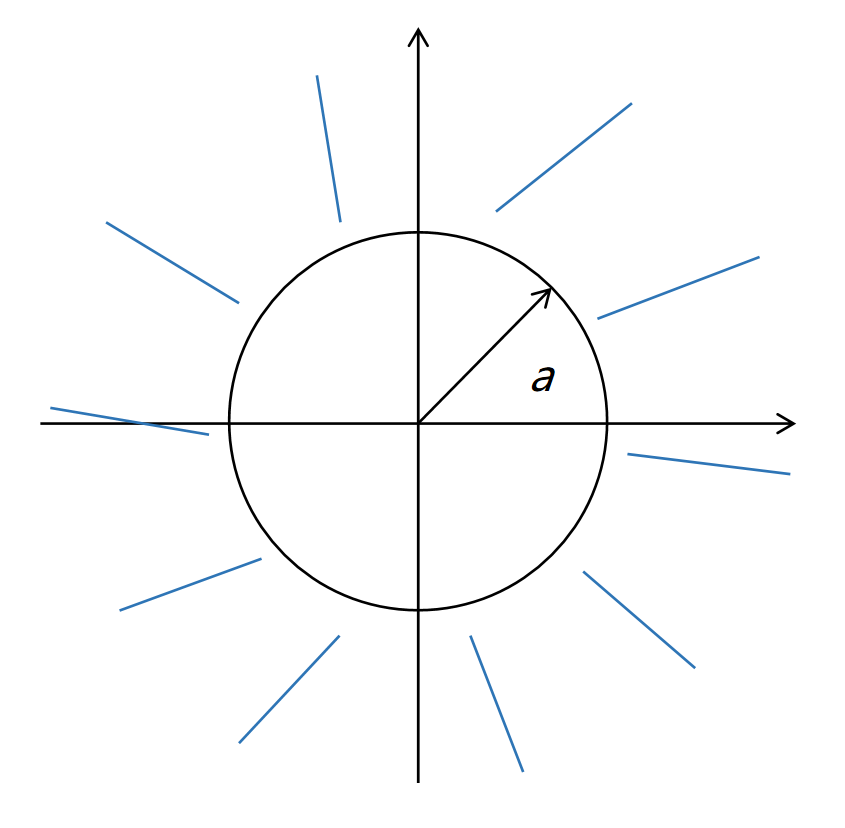
\includegraphics[scale=0.28]{例题收敛域.png}
\end{figure}

\newpage
\section{常用Z变换}
\begin{enumerate}[label=(\arabic*),itemindent=0pt,labelindent=\parindent,labelwidth=2em,labelsep=5pt,leftmargin=*]
  \item $\delta[k]\rightleftharpoons 1$
  \item $U[k]\rightleftharpoons \frac{z}{z-1}$
  \item $a^kU[k]\rightleftharpoons \frac{z}{z-a}$
  \item $e^{jbk}U[k]\rightleftharpoons \frac{z}{z-e^{jb}}$
\end{enumerate}\par

\section{Z变换的性质}
\begin{enumerate}[label=(\arabic*),itemindent=0pt,labelindent=\parindent,labelwidth=2em,labelsep=5pt,leftmargin=*]
  \item linear:if $f_1[k]\rightleftharpoons{F_1(z)}$,$f_2[k]\rightleftharpoons{F_2(z)}$ \par
        \begin{itemize}[label=,left=3em]
          \item than $af_1[k]+bf_2[k]\rightleftharpoons{aF_1(z)}+bF_2(z)$
        \end{itemize}
  \item 反转:if $f[k]\rightleftharpoons{F(z)}$ \par
        \begin{itemize}[label=,left=2.5em]
          \item than $f[-k]\rightleftharpoons{F(z^{-1})}$
        \end{itemize}
  \item 尺度变换:$a^kf[k]\rightleftharpoons{F(\frac{z}{a})}$
  \item 微分:$kf[k]\rightleftharpoons{(-z)\frac{\rm{d}}{{\rm{d}}z}F(z)}$ \par
        \begin{itemize}[label=,left=2.5em]
          \item $k^2f[k]\rightleftharpoons{(-z)\frac{\rm{d}}{{\rm{d}}z}[(-z)\frac{\rm{d}}{{\rm{d}}z}F(z)]}$
          \item $\cdots$
        \end{itemize}
  \item 卷积:$f_1[k]*f_2[k]\rightleftharpoons{F_1(z)\cdot F_2[z]}$
  \item $\bigstar$时移:$f(t\pm t_0)\stackrel{\mathscr{F}}{\leftrightharpoons}F(\omega)e^{\pm j\omega t_0}$ \par
        \begin{itemize}[label=,left=3.8em]
          \item $f(t-t_0)U(t-t_0)\stackrel{\mathscr{L}}{\leftrightharpoons}F(s)e^{-st_0}$(只考虑因果信号)
          \item \textcircled{1} \ 如果只考虑因果信号 \par
                \quad $f[k-m]\cdot U[k-m]\stackrel{\mathscr{Z}}{\leftrightharpoons}z^{-m}F(z) \quad k,m\in{\mathbb{Z^+}}$
          \item \textcircled{2} \ 对于“一般”信号的单边Z变换
        \end{itemize}
\end{enumerate}\par

\end{document}